%=======================================================================
%  IE 5311-001 (D01) Principles of Optimization
%  Homework 01 solutions
%
%  Packages used: geometry, amsmath, amssymb, amsthm, booktabs, array,
%  tikz (libraries: positioning, arrows.meta, calc).
%  All of these ship with Overleaf and with a full TeX Live install.
%  On a minimal install, tikz comes from texlive-pictures and booktabs
%  from texlive-latex-recommended.
%=======================================================================
\documentclass[11pt]{article}

\usepackage[margin=1in]{geometry}
\usepackage{amsmath}
\usepackage{amssymb}
\usepackage{amsthm}
\usepackage{booktabs}
\usepackage{array}
\usepackage{tikz}
\usetikzlibrary{positioning, arrows.meta, calc}

\DeclareMathOperator*{\minimize}{min}
\DeclareMathOperator*{\maximize}{max}

% node and box styles, black only
\tikzset{
  vtx/.style   = {draw, circle, minimum size=7mm, inner sep=0pt, font=\small},
  blk/.style   = {draw, rectangle, align=center, inner sep=4pt, font=\small,
                  minimum height=8mm},
  ar/.style    = {-{Stealth[length=2mm]}},
  used/.style  = {-{Stealth[length=2mm]}, line width=1.1pt},
  unused/.style= {-{Stealth[length=2mm]}, densely dashed, black!45},
  lbl/.style   = {font=\scriptsize, inner sep=1.5pt, fill=white},
}

\setlength{\parskip}{0.45em}
\setlength{\parindent}{0pt}

\begin{document}

%=======================================================================
\begin{center}
  {\large IE 5311-001 (D01) Principles of Optimization}\\[4pt]
  Lidivine Kengne\\[2pt]
  Homework01
\end{center}
\vspace{0.6em}

%=======================================================================
\section*{Problem 1.\quad Maya's Investment Plan \quad[20 pts]}
%=======================================================================

\subsection*{1.1\quad Time convention}

Let period $t$ index the BEGINNING of year $t$, so $t$ runs 1 to 5, and
let $t = 6$ denote the end of Year 5, the moment the objective is
measured. An instrument of term $L$ started at epoch $t$ matures at
epoch $t + L$ and is admissible only if $t + L \le 6$. Fixing this
convention first is what determines which instruments appear at which
epochs, and it is the step where the problem is most easily got wrong.

\begin{figure}[htbp]
\centering
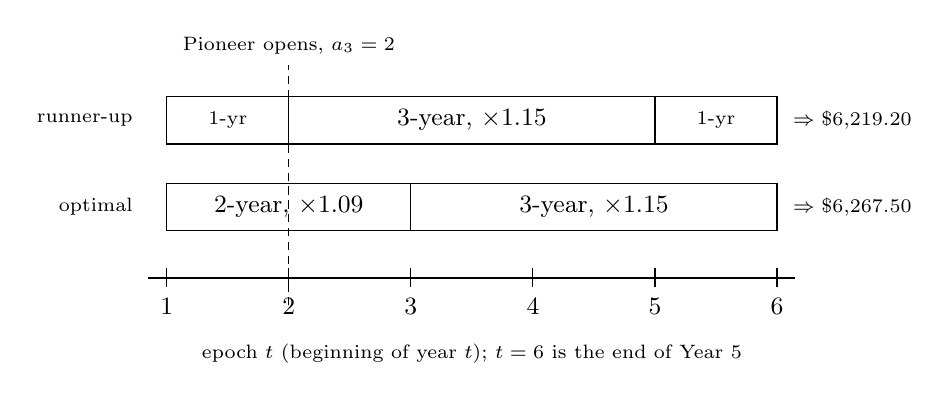
\begin{tikzpicture}[x=1.55cm, y=1cm]
  % timeline
  \draw[line width=0.9pt] (0.85,0) -- (6.15,0);
  \foreach \t in {1,2,3,4,5,6}{
    \draw (\t,0.12) -- (\t,-0.12);
    \node[below, font=\small] at (\t,-0.14) {$\t$};
  }
  \node[below, font=\scriptsize] at (3.5,-0.72)
    {epoch $t$ (beginning of year $t$); $t=6$ is the end of Year 5};
  % optimal plan
  \node[left, font=\scriptsize] at (0.80,0.90) {optimal};
  \draw (1,0.60) rectangle (3,1.20);
  \node[font=\small] at (2,0.90) {2-year, $\times 1.09$};
  \draw (3,0.60) rectangle (6,1.20);
  \node[font=\small] at (4.5,0.90) {3-year, $\times 1.15$};
  \node[right, font=\scriptsize] at (6.05,0.90) {$\Rightarrow \$6{,}267.50$};
  % runner up
  \node[left, font=\scriptsize] at (0.80,2.00) {runner-up};
  \draw (1,1.70) rectangle (2,2.30);
  \node[font=\scriptsize] at (1.5,2.00) {1-yr};
  \draw (2,1.70) rectangle (5,2.30);
  \node[font=\small] at (3.5,2.00) {3-year, $\times 1.15$};
  \draw (5,1.70) rectangle (6,2.30);
  \node[font=\scriptsize] at (5.5,2.00) {1-yr};
  \node[right, font=\scriptsize] at (6.05,2.00) {$\Rightarrow \$6{,}219.20$};
  % Pioneer availability
  \draw[densely dashed] (2,-0.35) -- (2,2.70);
  \node[above, font=\scriptsize] at (2,2.72) {Pioneer opens, $a_3 = 2$};
\end{tikzpicture}
\caption{Any admissible plan is a sequence of terms that exactly tiles
epochs 1 to 6. The three-year certificate cannot start before epoch 2,
which leaves it only two possible placements.}
\end{figure}

\subsection*{1.2\quad Sets}

\begin{center}
\begin{tabular}{@{}ll@{}}
\toprule
Symbol & Definition \\
\midrule
$T = \{1,\dots,5\}$ & Decision epochs, the beginning of each year \\
$K = \{1,2,3\}$     & Instrument types, indexed by their term in years \\
$A$                 & Admissible pairs $(t,k)$ with $t \ge a_k$ and $t + L_k \le 6$ \\
\bottomrule
\end{tabular}
\end{center}

\subsection*{1.3\quad Parameters}

\begin{center}
\begin{tabular}{@{}lll@{}}
\toprule
Symbol & Definition & Value \\
\midrule
$L_k$ & Term of instrument $k$                        & 1, 2, 3 years \\
$r_k$ & Total return multiplier over the full term    & 1.04, 1.09, 1.15 \\
$a_k$ & First epoch at which instrument $k$ is available & 1, 1, 2 \\
$B$   & Initial endowment                             & \$5,000 \\
$H$   & Horizon epoch                                 & 6 \\
\bottomrule
\end{tabular}
\end{center}

Pioneer's three-year certificate carries $a_3 = 2$ because it opens at
the beginning of Year 2. Combined with $t + 3 \le 6$ this leaves exactly
two admissible start epochs for it, $t = 2$ and $t = 3$.

\subsection*{1.4\quad Decision variables}

\[
  x_{t,k} \ge 0 \;=\; \text{dollars placed at epoch } t
  \text{ into an instrument of term } k
\]
\[
  w_t \ge 0 \;=\; \text{dollars held idle from epoch } t
  \text{ to epoch } t+1
\]

The idle-cash variables are included deliberately. Every instrument
earns a positive return, so they should all be zero at the optimum;
keeping them in the model makes full reinvestment a result rather than
an assumption baked into the formulation.

\subsection*{1.5\quad Model}

\begin{align}
  \maximize \quad
    & \sum_{(t,k) \in A \,:\, t + L_k = H} r_k\, x_{t,k} \;+\; w_5 \\[4pt]
  \text{s.t.} \quad
    & \sum_{k} x_{1,k} + w_1 = B
      && \text{epoch } 1 \\[2pt]
    & \sum_{k} x_{t,k} + w_t
      = \sum_{(s,k) \,:\, s + L_k = t} r_k\, x_{s,k} + w_{t-1}
      && t = 2,\dots,5 \\[2pt]
    & x_{t,k} \ge 0, \qquad w_t \ge 0 &&
\end{align}

The balance constraints are flow conservation on a timeline: what
matures at epoch $t$, plus whatever was carried forward, is exactly what
gets allocated at epoch $t$.

\subsection*{1.6\quad Result}

There are 11 admissible (epoch, instrument) pairs. The optimal value is
\$6,267.50.

\begin{center}
\begin{tabular}{@{}llrl@{}}
\toprule
Epoch & Term & Amount & Matures at \\
\midrule
1 & 2 years & \$5,000.00 & epoch 3 \\
3 & 3 years & \$5,450.00 & epoch 6 \\
\bottomrule
\end{tabular}
\end{center}

No idle cash is held at any epoch, which confirms the expectation above.
The plan is: a two-year deposit covering Years 1 and 2 returning
$5{,}000 \times 1.09 = \$5{,}450$, then the Pioneer three-year
certificate covering Years 3 to 5 returning
$5{,}450 \times 1.15 = \$6{,}267.50$.

\newpage
%=======================================================================
\section*{Problem 2.\quad Shortest and Longest $s$--$t$ Paths \quad[40 pts]}
%=======================================================================

\subsection*{2.1\quad Common sets and parameters}

\begin{center}
\begin{tabular}{@{}ll@{}}
\toprule
Symbol & Definition \\
\midrule
$V$ & Nodes, $|V| = 20$, with source $s$ and terminal $t$ \\
$A \subseteq V \times V$ & Directed arcs, a typical arc written $(i,j)$ \\
$\delta^{+}(i),\ \delta^{-}(i)$ & Out- and in-neighborhoods of node $i$ \\
$c_{ij}$ & Weight of arc $(i,j)$, drawn from $U[1,10]$ \\
$b_i$ & $+1$ at $s$, $-1$ at $t$, 0 at every other node \\
\bottomrule
\end{tabular}
\end{center}

\[
  x_{ij} = 1 \text{ if arc } (i,j) \text{ is used, 0 otherwise}
\]

\subsection*{2.2 (a)\quad Shortest path formulation}

\begin{align}
  \minimize \quad & \sum_{(i,j) \in A} c_{ij}\, x_{ij} \\[4pt]
  \text{s.t.} \quad
    & \sum_{j \in \delta^{+}(i)} x_{ij} \;-\; \sum_{j \in \delta^{-}(i)} x_{ji}
      = b_i && \forall\, i \in V \\[2pt]
    & x_{ij} \in \{0,1\} && \forall\, (i,j) \in A
\end{align}

Flow conservation alone suffices. A feasible integer point decomposes
into an $s$--$t$ path plus possibly some directed cycles that are
arc-disjoint from it; since every weight is at least 1, dropping a cycle
strictly lowers the objective, so no optimal solution contains one. This
argument depends on the weights being positive and would fail if
negative weights were allowed.

\subsection*{2.3 (b, c)\quad Integer model and LP relaxation}

The relaxation replaces the binary domain with $0 \le x_{ij} \le 1$. The
constraint matrix is the node-arc incidence matrix of a directed graph,
which is totally unimodular, and the right-hand side vector $b$ is
integral, so by the Hoffman and Kruskal theorem every vertex of the
relaxed polytope is integral. EP1 below develops this argument in full.

\subsection*{2.4 (d)\quad Comparison over the ten instances}

\begin{center}
\small
\begin{tabular}{@{}rrrrrrr@{}}
\toprule
Inst & $|A|$ & MIP objective & LP objective & MIP time (s) & LP time (s) & B\&B nodes \\
\midrule
1  & 59 & 10.4591 & 10.4591 & 0.0134 & 0.0003 & 1 \\
2  & 81 &  9.9972 &  9.9972 & 0.0130 & 0.0003 & 1 \\
3  & 61 &  8.3409 &  8.3409 & 0.0004 & 0.0003 & 0 \\
4  & 90 & 14.5495 & 14.5495 & 0.0018 & 0.0003 & 1 \\
5  & 73 & 22.2423 & 22.2423 & 0.0016 & 0.0002 & 1 \\
6  & 67 & 15.1332 & 15.1332 & 0.0016 & 0.0003 & 1 \\
7  & 58 & 13.6582 & 13.6582 & 0.0017 & 0.0003 & 1 \\
8  & 72 & 23.5501 & 23.5501 & 0.0017 & 0.0002 & 1 \\
9  & 80 &  9.8539 &  9.8539 & 0.0010 & 0.0002 & 1 \\
10 & 63 &  3.0157 &  3.0157 & 0.0016 & 0.0002 & 1 \\
\bottomrule
\end{tabular}
\end{center}

\textbf{Findings, on these ten instances.}\quad
The integrality gap was zero on all ten; the largest discrepancy was
$3.55 \times 10^{-15}$, floating-point noise rather than a gap. No arc
variable took a fractional value in any relaxed solution here. Branch
and bound explored at most one node, so the root relaxation was already
integral and no branching occurred on these instances. The relaxation
solved about 19 times faster in aggregate on this sample, though at
these sizes both models finish in a few milliseconds and the ratio is
dominated by fixed set-up overhead rather than search.

The zero gap is the part that generalizes, and not because of the
experiment: it follows from total unimodularity of the node-arc
incidence matrix, argued in EP1. The timing ratio does not generalize
and should not be read as a performance claim.

\subsection*{2.5 (a)\quad Longest simple path formulation}

\begin{align}
  \maximize \quad & \sum_{(i,j) \in A} c_{ij}\, x_{ij} \\[4pt]
  \text{s.t.} \quad
    & \sum_{j \in \delta^{+}(i)} x_{ij} \;-\; \sum_{j \in \delta^{-}(i)} x_{ji}
      = b_i && \forall\, i \in V \\[2pt]
    & \sum_{j \in \delta^{+}(i)} x_{ij} \;\le\; 1 && \forall\, i \in V \\[2pt]
    & \sum_{j \in \delta^{-}(i)} x_{ji} \;\le\; 1 && \forall\, i \in V \\[2pt]
    & \sum_{(i,j) \in A(S)} x_{ij} \;\le\; |S| - 1
      && \forall\, S \subseteq V \setminus \{s,t\},\ |S| \ge 2 \\[2pt]
    & x_{ij} \in \{0,1\} && \forall\, (i,j) \in A
\end{align}

where $A(S) = \{(i,j) \in A : i \in S,\ j \in S\}$ is the set of arcs
with both endpoints inside $S$.

\textbf{Why the in-degree family is there, and why it is not redundant.}\quad
It is tempting to drop it, on the grounds that flow conservation already
ties the two degrees together. That reasoning holds at every node except
one.

\begin{itemize}
\item For $i \notin \{s,t\}$: $b_i = 0$, so conservation gives
      $\mathrm{in}(i) = \mathrm{out}(i)$, and the out-degree limit already
      forces $\mathrm{in}(i) \le 1$. Redundant here.
\item For $s$: $b_s = +1$ gives $\mathrm{out}(s) = \mathrm{in}(s) + 1$, and
      with $\mathrm{out}(s) \le 1$ this forces $\mathrm{out}(s) = 1$ and
      $\mathrm{in}(s) = 0$. Redundant here too.
\item For $t$: $b_t = -1$ gives $\mathrm{in}(t) = \mathrm{out}(t) + 1$. The
      out-degree limit bounds this only by $\mathrm{in}(t) \le 2$.
      \textbf{Not redundant.} Without the in-degree constraint, $t$ may be
      entered twice and therefore lie on a cycle.
\end{itemize}

That single gap is what makes the index set of the subtour family
$S \subseteq V \setminus \{s,t\}$ rather than $S \subseteq V$. With the
in-degree family present, $\mathrm{in}(t) \le 1$ combines with
$\mathrm{in}(t) = \mathrm{out}(t) + 1$ to force $\mathrm{out}(t) = 0$, so
$t$ has no outgoing arc and cannot sit on a cycle. Neither can $s$, which
has no incoming arc. Every cycle therefore lies wholly inside
$V \setminus \{s,t\}$, and the family as written covers exactly the cycles
the separation routine can ever find.

Dropping the in-degree family and keeping the restricted index set would
be an error, and it was one: with out-degree only, the separation routine
generated 498 cuts over node sets containing $t$ across the ten
instances, none of which the restricted family authorizes. The written
model and the executed model have to agree, and they now do.

\textbf{What the subtour family is for.}\quad
The out-degree restriction enforces ``visiting each location at most
once''. The subtour family is mandatory here and this is the substantive
difference from the shortest path model. Under minimization a stray cycle
only adds cost and disappears on its own. Under maximization every cycle
adds weight for free, so the model without that family returns an
$s$--$t$ path plus as many disjoint cycles as the degree limits permit.

\begin{figure}[htbp]
\centering
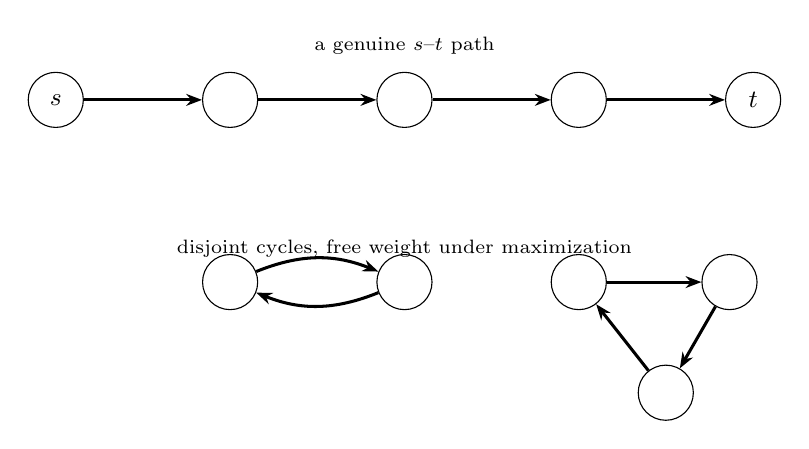
\begin{tikzpicture}[node distance=13mm and 15mm]
  \node[vtx] (s)  {$s$};
  \node[vtx, right=of s]  (p1) {};
  \node[vtx, right=of p1] (p2) {};
  \node[vtx, right=of p2] (p3) {};
  \node[vtx, right=of p3] (t)  {$t$};
  \draw[used] (s)--(p1);  \draw[used] (p1)--(p2);
  \draw[used] (p2)--(p3); \draw[used] (p3)--(t);
  \node[font=\scriptsize, above=1mm of p2] {a genuine $s$--$t$ path};

  \node[vtx, below=16mm of p1] (a1) {};
  \node[vtx, right=of a1]      (a2) {};
  \draw[used] (a1) to[bend left=22] (a2);
  \draw[used] (a2) to[bend left=22] (a1);

  \node[vtx, below=16mm of p3]        (b1) {};
  \node[vtx, right=12mm of b1]        (b2) {};
  \node[vtx, below right=9mm and 6mm of b1] (b3) {};
  \draw[used] (b1)--(b2);  \draw[used] (b2)--(b3);  \draw[used] (b3)--(b1);

  \node[font=\scriptsize, below=13mm of p2]
    {disjoint cycles, free weight under maximization};
\end{tikzpicture}
\caption{A feasible point of the model with the subtour family removed.
Conservation and both degree limits hold, yet the solution is not a
path. Both degree limits also confine every such cycle to
$V \setminus \{s,t\}$, which is why the family is indexed over that set.}
\end{figure}

\textbf{Measured on instance 1.}\quad
The master problem with no subtour constraint returns 107.1629,
selecting 19 arcs that contain three separate cycles: $\{11,15\}$,
$\{17,18,2\}$ and $\{1,10,16,12,9,7,14\}$. None touches $s = 0$ or
$t = 19$, as the argument above requires. The true longest simple path
is 98.6059, so the unconstrained master overstates it by 8.5570 and its
answer is not a path at all.

\subsection*{2.6 (b, c)\quad Two generation strategies}

\textbf{Constraint generation.}\quad
Solve the master to proven optimality with the subtour constraints found
so far. Inspect the incumbent, detect every simple cycle among the
selected arcs, add the corresponding constraint for each, and re-solve
from scratch. Each round is a complete branch-and-bound run.

\textbf{Lazy constraints.}\quad
Run a single branch-and-bound search. A callback fires at every
integer-feasible incumbent (Gurobi's \texttt{MIPSOL} event), detects
cycles in that incumbent, and injects the violated constraints through
\texttt{cbLazy}. The search continues from where it was, keeping its
tree, bounds and pseudo-costs.

\begin{figure}[htbp]
\centering
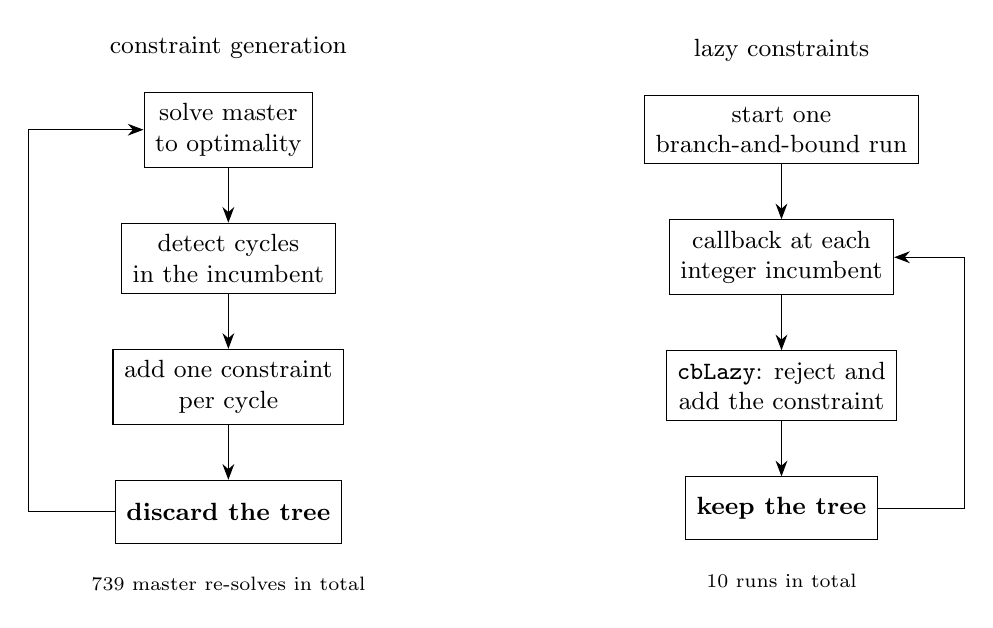
\begin{tikzpicture}[node distance=7mm]
  % ---- left: constraint generation ----
  \node[blk] (cg1) {solve master\\to optimality};
  \node[blk, below=of cg1] (cg2) {detect cycles\\in the incumbent};
  \node[blk, below=of cg2] (cg3) {add one constraint\\per cycle};
  \node[blk, below=of cg3] (cg4) {\textbf{discard the tree}};
  \draw[ar] (cg1)--(cg2);  \draw[ar] (cg2)--(cg3);  \draw[ar] (cg3)--(cg4);
  \draw[ar] (cg4.west) -- ++(-1.1,0) |- (cg1.west);
  \node[font=\small, above=3mm of cg1] {constraint generation};
  \node[font=\scriptsize, below=3mm of cg4] {739 master re-solves in total};

  % ---- right: lazy constraints ----
  \node[blk, right=42mm of cg1] (lz1) {start one\\branch-and-bound run};
  \node[blk, below=of lz1] (lz2) {callback at each\\integer incumbent};
  \node[blk, below=of lz2] (lz3) {\texttt{cbLazy}: reject and\\add the constraint};
  \node[blk, below=of lz3] (lz4) {\textbf{keep the tree}};
  \draw[ar] (lz1)--(lz2);  \draw[ar] (lz2)--(lz3);  \draw[ar] (lz3)--(lz4);
  \draw[ar] (lz4.east) -- ++(1.1,0) |- (lz2.east);
  \node[font=\small, above=3mm of lz1] {lazy constraints};
  \node[font=\scriptsize, below=3mm of lz4] {10 runs in total};
\end{tikzpicture}
\caption{The difference is where the work is thrown away. Constraint
generation rebuilds the search tree every round; the lazy callback keeps
one tree and its accumulated bounds.}
\end{figure}

\subsection*{2.7 (d)\quad Comparison over the ten instances}

\begin{center}
\small
\begin{tabular}{@{}rrrrrrrr@{}}
\toprule
Inst & CG objective & Lazy objective & CG time (s) & Lazy time (s)
     & CG rounds & CG cuts & Lazy cuts \\
\midrule
1  &  98.6059 &  98.6059 &  0.0138 & 0.0230 &   3 &   4 &  12 \\
2  &  96.4163 &  96.4163 &  0.0471 & 0.0143 &   7 &  10 &  17 \\
3  &   8.3409 &   8.3409 & 12.2977 & 0.1103 & 215 & 227 & 227 \\
4  & 135.2684 & 135.2684 &  0.0027 & 0.0018 &   1 &   0 &   0 \\
5  & 104.4747 & 104.4747 &  0.0247 & 0.0214 &   5 &   4 &  12 \\
6  & 121.4952 & 121.4952 &  0.0069 & 0.0030 &   2 &   1 &   1 \\
7  &  92.6552 &  92.6552 &  0.0327 & 0.0119 &   7 &   6 &   7 \\
8  & 120.5135 & 120.5135 &  0.0116 & 0.0036 &   4 &   7 &   8 \\
9  &  86.8009 &  86.8009 &  0.1103 & 0.0419 &  10 &  16 &  30 \\
10 &  87.6195 &  87.6195 &  0.0025 & 0.0030 &   1 &   0 &   4 \\
\bottomrule
\end{tabular}
\end{center}

\begin{figure}[htbp]
\centering
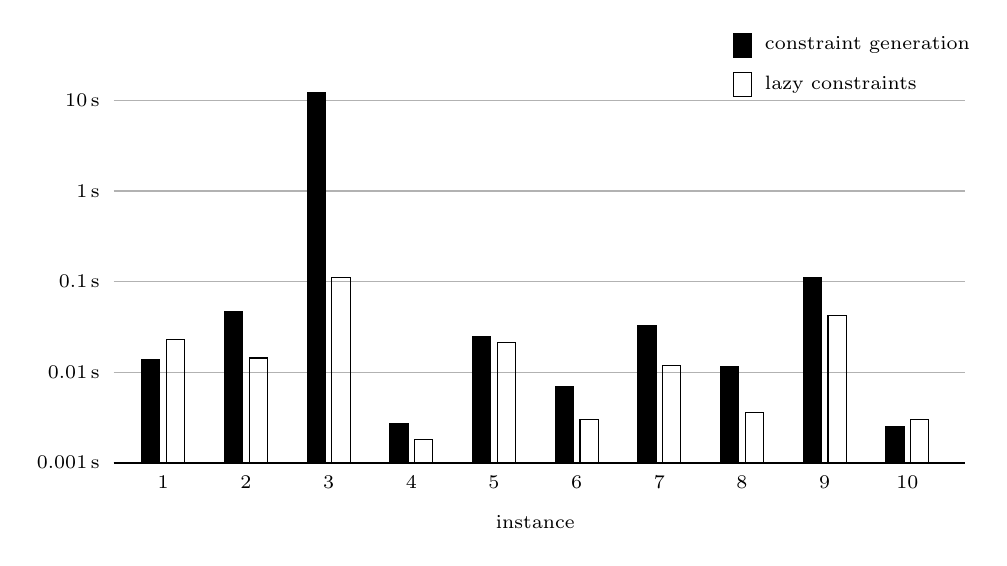
\begin{tikzpicture}[x=1.05cm, y=1cm]
  \foreach \y/\lab in {0.000/0.001, 1.150/0.01, 2.300/0.1, 3.450/1, 4.600/10}{
    \draw[black!30] (0.4,\y) -- (10.7,\y);
    \node[left, font=\scriptsize] at (0.35,\y) {\lab\,s};
  }
  \draw[line width=0.8pt] (0.4,0) -- (10.7,0);
  \foreach \x/\h in {1/1.311, 2/1.924, 3/4.703, 4/0.496, 5/1.602,
                     6/0.965, 7/1.742, 8/1.224, 9/2.349, 10/0.458}{
    \draw[fill=black] (\x-0.26,0) rectangle (\x-0.04,\h);
  }
  \foreach \x/\h in {1/1.566, 2/1.329, 3/2.349, 4/0.294, 5/1.530,
                     6/0.549, 7/1.237, 8/0.640, 9/1.866, 10/0.549}{
    \draw (\x+0.04,0) rectangle (\x+0.26,\h);
  }
  \foreach \x in {1,...,10}{
    \node[below, font=\scriptsize] at (\x,-0.05) {\x};
  }
  \node[below, font=\scriptsize] at (5.5,-0.55) {instance};
  \draw[fill=black] (7.9,5.15) rectangle (8.12,5.45);
  \node[right, font=\scriptsize] at (8.16,5.30) {constraint generation};
  \draw (7.9,4.65) rectangle (8.12,4.95);
  \node[right, font=\scriptsize] at (8.16,4.80) {lazy constraints};
\end{tikzpicture}
\caption{Solution time per instance, logarithmic vertical axis. Instance
3 dominates the picture and the aggregate; on the other nine the two
methods are within a small factor of each other, and on instances 1 and
10 constraint generation was the faster of the two.}
\end{figure}

\textbf{Findings, on these ten instances.}\quad
Both methods returned identical objective values on all ten, as they
must, since both converge to the same fully-constrained problem.

The aggregate timing ratio is 53.6 to 1 in favour of the lazy method,
and that single number is misleading enough to be worth unpacking.
Instance 3 accounts for 98\% of the total constraint-generation time.
Excluding it, the aggregate ratio falls to 2.0 to 1. The median
per-instance ratio is 2.5 to 1. On instances 1 and 10 the lazy method
was actually the \emph{slower} of the two, by factors of 1.7 and 1.2,
because at that size the callback overhead is not repaid.

So what this experiment supports is a conditional claim: when many
separation rounds are needed, reusing one search tree pays, and the
payoff grows with the number of rounds. Instance 3 needed 215 rounds and
showed a 111 to 1 gap; instances 4 and 10 needed one round each and
showed none. What it does not support is a claim that the lazy method is
uniformly faster, or any statement about how the gap behaves at sizes
not tested here.

Constraint generation required 255 complete master re-solves in total
across the ten instances, against ten branch-and-bound runs for the lazy
method.

\textbf{The instance that surprised me.}\quad
Instance 3 was the worst case for constraint generation, needing 215
rounds, yet its optimal value 8.3409 is identical to its shortest path
value. I expected the hardest instance to be a dense one with many
competing paths. Enumerating its simple $s$--$t$ paths explains it:
instance 3 has exactly one, namely $0 \rightarrow 11 \rightarrow 19$, so
the shortest and longest paths must coincide. The 215 rounds were not
spent choosing between paths. They were spent eliminating cycles
elsewhere in the graph before the model was forced onto the only path
available. On this sample, difficulty tracked the number of cycles the
master could chase rather than the number of paths that competed.

\subsection*{2.8 (e)\quad Algorithmic differences}

The difference is where the work is thrown away.

Constraint generation treats the solver as a black box. Every round
starts a fresh branch-and-bound search that must rediscover the same
bounds, the same branching decisions and the same cuts as the previous
round, only to be told about one more constraint at the end. The cost
per round grows as the master accumulates constraints, so the later
rounds are the expensive ones.

Lazy constraints put the separation inside the search. One tree is built
and kept. When an incumbent turns out to violate a constraint, it is
rejected and the constraint is added, but the tree, its bounds, its
pseudo-costs and its already-proven prunings all survive.

That mechanism explains the shape of the results above rather than a
single headline number. The saving is proportional to how many rounds
would otherwise be repeated, which is why instance 3 at 215 rounds shows
a large gap and the single-round instances show none at all.

Two costs come with the lazy method, and they are what the two losing
instances are made of. The callback runs inside the solver, so
separation must be fast, and a slow detection routine is paid at every
incumbent. The solver must also be told in advance
(\texttt{LazyConstraints = 1}), which disables some presolve reductions
that would otherwise be unsafe, since presolve cannot know about
constraints that do not exist yet. Constraint generation keeps full
presolve on every round. When few rounds are needed, those fixed costs
are not recovered, which is what happened on instances 1 and 10.

\newpage
%=======================================================================
\section*{Problem 3.\quad GlobalLogix Distribution Network \quad[45 pts]}
%=======================================================================

\subsection*{3.1\quad Sets}

\begin{center}
\begin{tabular}{@{}ll@{}}
\toprule
Symbol & Definition \\
\midrule
$F = \{f_1, f_2\}$        & Factories \\
$D = \{d_1, d_2\}$        & Distribution centres, pure transshipment \\
$S = \{s_1, s_2, s_3\}$   & Stores \\
$N = F \cup D \cup S$     & All nodes, indexed by $i$ and $j$ \\
$A_1 = F \times D$        & Factory-to-DC arcs \\
$A_2 = D \times S$        & DC-to-store arcs \\
$A = A_1 \cup A_2$        & All arcs \\
\bottomrule
\end{tabular}
\end{center}

\subsection*{3.2\quad Parameters}

\begin{center}
\begin{tabular}{@{}lll@{}}
\toprule
Symbol & Definition & Units \\
\midrule
$b_i$ & Net supply: $+70$ at $f_1$, $+50$ at $f_2$,
        $-40/-45/-35$ at stores, 0 at DCs & units \\
$u_{ij}$ & Capacity of arc $(i,j)$ & units \\
$c_{ij}$ & Cost per unit shipped on arc $(i,j)$ & \$/unit \\
\bottomrule
\end{tabular}
\end{center}

Total supply is 120 and total demand is 120, so the $b_i$ sum to zero
and a feasible flow can exist. The DCs carry $b_i = 0$, which is exactly
what ``do not generate or consume products'' means in the model.

\begin{figure}[htbp]
\centering
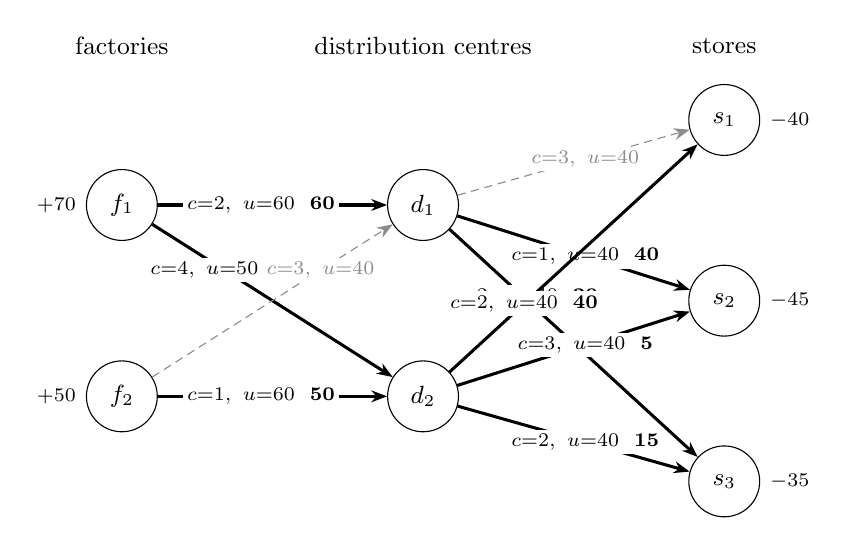
\begin{tikzpicture}[x=2.55cm, y=1.35cm]
  % nodes
  \node[vtx, minimum size=9mm] (f1) at (0, 2.1) {$f_1$};
  \node[vtx, minimum size=9mm] (f2) at (0, 0.3) {$f_2$};
  \node[vtx, minimum size=9mm] (d1) at (1.5, 2.1) {$d_1$};
  \node[vtx, minimum size=9mm] (d2) at (1.5, 0.3) {$d_2$};
  \node[vtx, minimum size=9mm] (s1) at (3.0, 2.9) {$s_1$};
  \node[vtx, minimum size=9mm] (s2) at (3.0, 1.2) {$s_2$};
  \node[vtx, minimum size=9mm] (s3) at (3.0,-0.5) {$s_3$};
  % supply and demand annotations
  \node[left,  font=\scriptsize] at (-0.18, 2.1) {$+70$};
  \node[left,  font=\scriptsize] at (-0.18, 0.3) {$+50$};
  \node[right, font=\scriptsize] at ( 3.18, 2.9) {$-40$};
  \node[right, font=\scriptsize] at ( 3.18, 1.2) {$-45$};
  \node[right, font=\scriptsize] at ( 3.18,-0.5) {$-35$};
  % factory to DC
  \draw[used]   (f1) -- node[lbl, pos=0.45] {$c{=}2,\ u{=}60$\ \ \textbf{60}} (d1);
  \draw[used]   (f1) -- node[lbl, pos=0.30] {$c{=}4,\ u{=}50$\ \ \textbf{10}} (d2);
  \draw[unused] (f2) -- node[lbl, pos=0.70] {$c{=}3,\ u{=}40$} (d1);
  \draw[used]   (f2) -- node[lbl, pos=0.45] {$c{=}1,\ u{=}60$\ \ \textbf{50}} (d2);
  % DC to store
  \draw[unused] (d1) -- node[lbl, pos=0.55] {$c{=}3,\ u{=}40$} (s1);
  \draw[used]   (d1) -- node[lbl, pos=0.55] {$c{=}1,\ u{=}40$\ \ \textbf{40}} (s2);
  \draw[used]   (d1) -- node[lbl, pos=0.30] {$c{=}2,\ u{=}40$\ \ \textbf{20}} (s3);
  \draw[used]   (d2) -- node[lbl, pos=0.30] {$c{=}2,\ u{=}40$\ \ \textbf{40}} (s1);
  \draw[used]   (d2) -- node[lbl, pos=0.55] {$c{=}3,\ u{=}40$\ \ \textbf{5}}  (s2);
  \draw[used]   (d2) -- node[lbl, pos=0.55] {$c{=}2,\ u{=}40$\ \ \textbf{15}} (s3);
  % column labels
  \node[font=\small] at (0,  3.6) {factories};
  \node[font=\small] at (1.5,3.6) {distribution centres};
  \node[font=\small] at (3.0,3.6) {stores};
\end{tikzpicture}
\caption{The network with cost and capacity on every arc. Bold numbers
are the optimal flow. Dashed arcs carry nothing at the optimum. Total
cost \$415.00. Arcs $(f_1,d_1)$, $(d_1,s_2)$ and $(d_2,s_1)$ run at
capacity.}
\end{figure}

\subsection*{3.3 (1)\quad Deterministic formulation}

\begin{align}
  \minimize \quad & \sum_{(i,j) \in A} c_{ij}\, x_{ij} \\[4pt]
  \text{s.t.} \quad
    & \sum_{j \,:\, (i,j) \in A} x_{ij} \;-\; \sum_{j \,:\, (j,i) \in A} x_{ji}
      = b_i && \forall\, i \in N \\[2pt]
    & 0 \le x_{ij} \le u_{ij} && \forall\, (i,j) \in A
\end{align}

\textbf{Result.}\quad Minimum cost \$415.00.

\begin{center}
\begin{tabular}{@{}lrrrrl@{}}
\toprule
Arc & Flow & Capacity & Cost/unit & Cost & Status \\
\midrule
$(f_1, d_1)$ & 60.0 & 60 & 2 & 120.0 & at capacity \\
$(f_1, d_2)$ & 10.0 & 50 & 4 &  40.0 & \\
$(f_2, d_2)$ & 50.0 & 60 & 1 &  50.0 & \\
$(d_1, s_2)$ & 40.0 & 40 & 1 &  40.0 & at capacity \\
$(d_1, s_3)$ & 20.0 & 40 & 2 &  40.0 & \\
$(d_2, s_1)$ & 40.0 & 40 & 2 &  80.0 & at capacity \\
$(d_2, s_2)$ &  5.0 & 40 & 3 &  15.0 & \\
$(d_2, s_3)$ & 15.0 & 40 & 2 &  30.0 & \\
\bottomrule
\end{tabular}
\end{center}

\subsection*{3.4 (2a)\quad Robust formulation, worst case}

The uncertainty set is a box: each $c_{ij}$ lies in
$[0.99 c_{ij},\, 1.01 c_{ij}]$ and each $u_{ij}$ in
$[0.99 u_{ij},\, 1.01 u_{ij}]$. The robust problem is
\[
  \min_{x} \ \max_{(c,u) \in \mathcal{U}} \ \sum_{(i,j) \in A} c_{ij} x_{ij}
\]
subject to flow conservation and to the capacity bound holding for every
realization. Both inner problems have closed-form answers, so no inner
optimization is needed. Cost enters the objective with a positive
coefficient and $x \ge 0$, so the worst case is the upper cost bound.
The capacity constraint must hold for every realization, so the binding
bound is the lowest capacity. The robust counterpart is therefore an
ordinary linear program:

\begin{align}
  \minimize \quad & \sum_{(i,j) \in A} 1.01\, c_{ij}\, x_{ij} \\[2pt]
  \text{s.t.} \quad & \text{flow conservation as above} \\[2pt]
    & 0 \le x_{ij} \le 0.99\, u_{ij} && \forall\, (i,j) \in A
\end{align}

\textbf{Result.}\quad Worst-case cost \$421.57, a premium of \$6.57 or
$1.58\%$ over the deterministic solution.

\textbf{What surprised me.}\quad
I expected the robust routing to match the deterministic routing with a
$1\%$ price mark-up, since a uniform $1.01$ scaling of all costs cannot
change which route is cheapest. It does not match. The robust plan opens
a new arc, $(d_1, s_1)$, carrying 0.4 units. The reason is the capacity
side, not the cost side: shrinking every capacity by $1\%$ removes 0.4
units of throughput from $(d_2, s_1)$, which was at its limit, and that
shortfall has to be picked up somewhere. Worst-case protection changed
the structure of the plan, not just its price. Note also that $1.58\%$
exceeds the $1\%$ cost inflation, and the excess is precisely the cost
of that forced rerouting.

\subsection*{3.5 (2b)\quad Stochastic formulation, average case}

A stochastic program differs from a deterministic one only if some
decision must be committed before the uncertainty is observed. The
problem statement does not say which decisions those are, so the split
has to be assumed, and the assumption drives the entire model. I state
it explicitly rather than leaving it implicit in the notation.

\textbf{Assumption (decision timing).}\quad
\emph{The factory-to-DC shipments $x_{ij}$, $(i,j) \in A_1$, are
committed before the realization $(c^{\omega}, u^{\omega})$ is observed.
The DC-to-store deliveries $y^{\omega}_{jk}$, $(j,k) \in A_2$, and any
unmet demand $v^{\omega}_{k}$ are decided after it is observed.}

The reading behind it: long-haul factory-to-DC movements are planned and
dispatched on a longer cycle than local DC-to-store deliveries, so by the
time the day's realized costs and capacities are known, the inbound
shipment is already in transit and cannot be redirected. Local
deliveries still can be.

Two consequences follow, and both are worth flagging because they are
where the assumption bites.

\begin{itemize}
\item The first-stage capacity bound must hold in every scenario, since
      $x$ is fixed before $u^{\omega}$ is seen. That is why it reads
      $x_{ij} \le 0.99\, u_{ij}$, a worst-case bound sitting inside an
      otherwise average-case model.
\item If the split were reversed, or if every decision were deferred
      until after the realization, the model would collapse to a
      collection of independent deterministic problems and the stochastic
      formulation would carry no information the nominal one does not.
\end{itemize}

\begin{figure}[htbp]
\centering
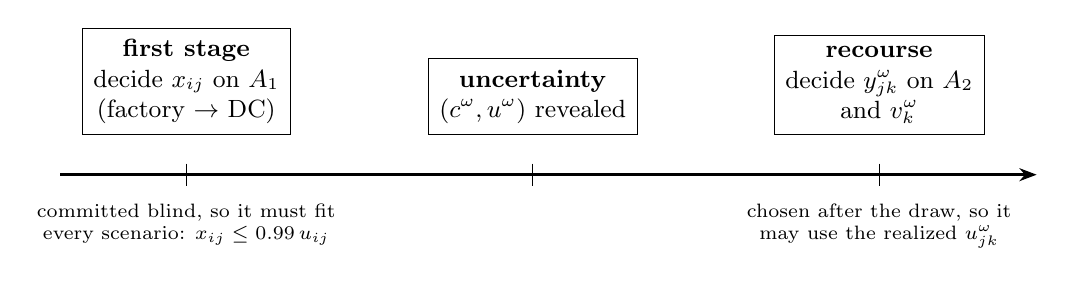
\begin{tikzpicture}[x=1cm, y=1cm]
  \draw[line width=0.9pt, -{Stealth[length=2.2mm]}] (0,0) -- (12.4,0);
  \foreach \x in {1.6, 6.0, 10.4}{ \draw (\x,0.14) -- (\x,-0.14); }
  \node[blk, above=5mm of {(1.6,0)}, anchor=south]
    {\textbf{first stage}\\decide $x_{ij}$ on $A_1$\\(factory $\to$ DC)};
  \node[blk, above=5mm of {(6.0,0)}, anchor=south]
    {\textbf{uncertainty}\\$(c^{\omega}, u^{\omega})$ revealed};
  \node[blk, above=5mm of {(10.4,0)}, anchor=south]
    {\textbf{recourse}\\decide $y^{\omega}_{jk}$ on $A_2$\\and $v^{\omega}_k$};
  \node[below, font=\scriptsize, align=center] at (1.6,-0.25)
    {committed blind, so it must fit\\every scenario: $x_{ij} \le 0.99\, u_{ij}$};
  \node[below, font=\scriptsize, align=center] at (10.4,-0.25)
    {chosen after the draw, so it\\may use the realized $u^{\omega}_{jk}$};
\end{tikzpicture}
\caption{The decision-timing assumption drawn out. Only the first-stage
commitment is exposed to the uncertainty, and that exposure is the sole
reason the stochastic model differs from the nominal one.}
\end{figure}

\textbf{The unmet-demand penalty.}\quad
The recourse stage needs a penalty $p$ per unit of unmet demand,
otherwise the second stage can be infeasible in scenarios where realized
capacity cannot carry the committed flow. Its value is not free: $p$ has
to exceed the most expensive way to actually deliver a unit, or the model
would prefer paying the penalty to shipping. Over all factory--DC--store
routes the dearest delivered unit is $f_1 \to d_2 \to s_2$ at
$4 + 3 = \$7$, so any $p > 7$ makes delivery strictly preferred.

I used $p = 50$. The choice does not affect the answer, which is the
point of checking it: at 150 scenarios the expected cost is
\$416.4478 at $p = 7$, \$416.4624 at $p = 8$, and \$416.4624 at
$p = 20$, $50$ and $500$ alike. Above the \$7 threshold the expected
unmet demand is zero, so the penalty is never actually paid and its
magnitude never enters the objective. Below the threshold it does bite:
at $p = 5$ the model abandons 10.6 units of demand on average, and at
$p = 1$ it ships nothing at all.

\begin{center}
\begin{tabular}{@{}ll@{}}
\toprule
Symbol & Definition \\
\midrule
$\Omega$ & Scenario set, indexed by $\omega$, with probability
           $\pi_{\omega} = 1/|\Omega|$ \\
$c^{\omega}, u^{\omega}$ & Cost and capacity realized in scenario $\omega$ \\
$p$ & Penalty per unit of unmet demand, \$/unit \\
\bottomrule
\end{tabular}
\end{center}

\begin{align}
  \minimize \quad
    & \sum_{(i,j) \in A_1} c_{ij}\, x_{ij}
      + \sum_{\omega \in \Omega} \pi_{\omega}
        \Bigl[ \sum_{(j,k) \in A_2} c^{\omega}_{jk}\, y^{\omega}_{jk}
             + p \sum_{k \in S} v^{\omega}_{k} \Bigr] \\[4pt]
  \text{s.t.} \quad
    & \sum_{j} x_{ij} \le \text{supply at } i && \forall\, i \in F \\[2pt]
    & x_{ij} \le 0.99\, u_{ij} && \forall\, (i,j) \in A_1 \\[2pt]
    & \sum_{i} x_{ij} = \sum_{k} y^{\omega}_{jk}
      && \forall\, j \in D,\ \omega \in \Omega \\[2pt]
    & \sum_{j} y^{\omega}_{jk} + v^{\omega}_{k} = \text{demand at } k
      && \forall\, k \in S,\ \omega \in \Omega \\[2pt]
    & 0 \le y^{\omega}_{jk} \le u^{\omega}_{jk}, \quad v^{\omega}_{k} \ge 0
      && \forall\, (j,k) \in A_2,\ \omega \in \Omega
\end{align}

The first-stage capacity bound uses $0.99\, u_{ij}$ rather than a
scenario value. A shipment committed before the capacity is observed
must fit in every realization, so that bound is robust even inside a
stochastic model.

\subsection*{3.6 (2b continued)\quad Solution and the solver ceiling}

Each parameter is drawn independently as $+1\%$ or $-1\%$ with
probability one half, matching ``equally likely''. The model has
$4 + 9|\Omega|$ variables and $2 + 11|\Omega|$ constraints, so it exceeds
the 2,000-variable Gurobi size-limited licence beyond $|\Omega| = 181$. The
larger samples were therefore solved with CBC through PuLP.

\begin{center}
\begin{tabular}{@{}rlrrr@{}}
\toprule
Scenarios & Solver & Expected cost & $\mathbb{E}[\text{unmet}]$ & Variables \\
\midrule
1     & Gurobi & \$415.58 & 0.0000 & 13 \\
10    & Gurobi & \$416.12 & 0.0000 & 94 \\
50    & Gurobi & \$416.62 & 0.0000 & 454 \\
150   & Gurobi & \$416.46 & 0.0000 & 1,354 \\
500   & CBC    & \$416.40 & 0.0000 & 4,504 \\
2,000 & CBC    & \$416.44 & 0.0000 & 18,004 \\
\bottomrule
\end{tabular}
\end{center}

\textbf{Findings.}\quad
The expected cost settles around \$416.44, between the deterministic
\$415.00 and the robust \$421.57. That ordering is the sanity check and
it holds: average-case protection costs less than worst-case protection
and more than assuming nothing goes wrong. Expected unmet demand is zero
at every sample size, because a $1\%$ capacity swing is small enough
that the recourse stage always absorbs it.

\textbf{Something worth stating explicitly.}\quad
The cost randomness contributes nothing.
$\mathbb{E}[c_{ij}] = \tfrac{1}{2}(0.99 c_{ij}) + \tfrac{1}{2}(1.01 c_{ij})
= c_{ij}$ exactly, and expectation is linear, so replacing every cost by
its mean reproduces the deterministic problem and its \$415.00 answer to
the cent. Only the capacity randomness makes the stochastic model differ
from the nominal one, and only because the first-stage shipment is
committed before capacity is observed. A symmetric mean-zero
perturbation of objective coefficients alone never changes a risk-neutral
stochastic linear program.

\subsection*{3.7 (3)\quad Multicommodity extension}

Add a commodity index. Let $P$ be the set of product lines, indexed by
$q$, with $P = \{\text{Standard}, \text{Premium}\}$ in the stated case.

\begin{center}
\begin{tabular}{@{}ll@{}}
\toprule
Symbol & Definition \\
\midrule
$P$ & Product lines, indexed by $q$ \\
$b_i^{q}$ & Net supply of product $q$ at node $i$, units; positive at
            factories, negative at stores, zero at DCs \\
$c_{ij}^{q}$ & Cost per unit of product $q$ shipped on arc $(i,j)$, \$/unit \\
$u_{ij}$ & Capacity of arc $(i,j)$, SHARED across products, units \\
\bottomrule
\end{tabular}
\end{center}

\[
  x_{ij}^{q} \ge 0 \;=\; \text{units of product } q
  \text{ shipped on arc } (i,j)
\]

\begin{align}
  \minimize \quad & \sum_{q \in P} \sum_{(i,j) \in A} c_{ij}^{q}\, x_{ij}^{q} \\[4pt]
  \text{s.t.} \quad
    & \sum_{j \,:\, (i,j) \in A} x_{ij}^{q}
      \;-\; \sum_{j \,:\, (j,i) \in A} x_{ji}^{q} = b_i^{q}
      && \forall\, i \in N,\ q \in P \\[2pt]
    & \sum_{q \in P} x_{ij}^{q} \le u_{ij}
      && \forall\, (i,j) \in A \\[2pt]
    & x_{ij}^{q} \ge 0 && \forall\, (i,j) \in A,\ q \in P
\end{align}

The structural point is the difference between the two constraint
families. Flow conservation is written once per product, so it
decomposes: without the second family the problem would split into
$|P|$ independent single-commodity problems, each solvable separately.
The capacity constraint is written once per arc and sums across
products, and it is the only thing coupling them. That single family is
what makes multicommodity flow harder than $|P|$ separate flow problems,
and it is also why the linear relaxation of a multicommodity integer
flow problem is generally not integral even though each single-commodity
piece would be.

\newpage
%=======================================================================
\section*{Problem 4.\quad Sudoku \quad[30 pts]}
%=======================================================================

\subsection*{4.1 (1)\quad Formulation with linear constraints and binary variables}

\begin{center}
\begin{tabular}{@{}ll@{}}
\toprule
Symbol & Definition \\
\midrule
$R = C = V = \{1,\dots,9\}$ & Rows, columns, digit values \\
$B = \{1,\dots,9\}$ & The nine $3 \times 3$ sub-blocks \\
$\mathrm{cells}(b)$ & The nine cells belonging to block $b$ \\
$G$ & Given clues: $(r,c,v) \in G$ means cell $(r,c)$ is pre-filled with digit $v$ \\
\bottomrule
\end{tabular}
\end{center}

\[
  x_{r,c,v} \in \{0,1\} \;=\; 1 \text{ if cell } (r,c) \text{ holds digit } v
\]

The problem is pure feasibility, so a constant objective is used. Every
rule becomes an equality.

\begin{align}
  & \sum_{v \in V} x_{r,c,v} = 1 && \forall\, r \in R,\ c \in C \\[2pt]
  & \sum_{c \in C} x_{r,c,v} = 1 && \forall\, r \in R,\ v \in V \\[2pt]
  & \sum_{r \in R} x_{r,c,v} = 1 && \forall\, c \in C,\ v \in V \\[2pt]
  & \sum_{(r,c) \in \mathrm{cells}(b)} x_{r,c,v} = 1 && \forall\, b \in B,\ v \in V \\[2pt]
  & x_{r,c,v} = 1 && \forall\, (r,c,v) \in G
\end{align}

All four structural families are needed and none is redundant. The first
says each cell holds exactly one digit; it says nothing about
uniqueness. The other three are the three uniqueness rules, one per
direction. Writing them as equalities rather than $\le 1$ is what makes
the count work: nine cells and nine digits means ``at most once'' and
``exactly once'' coincide, and equalities give the solver tighter
information.

\textbf{Model size.}\quad 729 binary variables and 346 constraints,
being 81 cell equations, 81 row, 81 column and 81 block equations, plus
22 clue fixings.

\subsection*{4.2 (2, 3)\quad Solution of the given instance}

The instance carries 22 clues. For reference, 17 is the proven minimum
number of clues for a uniquely solvable Sudoku (McGuire, Tugemann and
Civario, 2012), so 22 is above that threshold but says nothing by itself
about whether this particular instance is unique.

\begin{figure}[htbp]
\centering
\begin{minipage}{0.47\textwidth}
\centering
  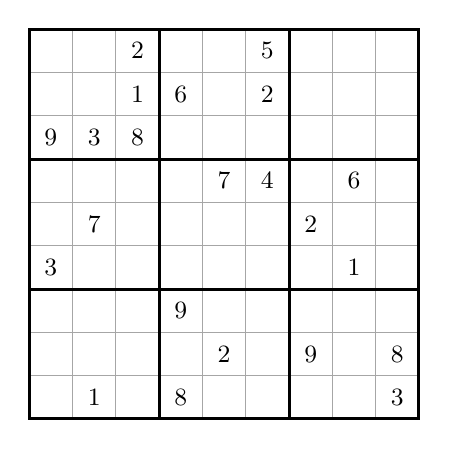
\begin{tikzpicture}[scale=0.55, every node/.style={font=\small}]
    \draw[step=1, black!35, thin] (0,0) grid (9,9);
    \draw[line width=1.1pt] (0,0) rectangle (9,9);
    \draw[line width=1.1pt] (3,0)--(3,9);  \draw[line width=1.1pt] (6,0)--(6,9);
    \draw[line width=1.1pt] (0,3)--(9,3);  \draw[line width=1.1pt] (0,6)--(9,6);
    \node at (2.5,8.5) {2};
    \node at (5.5,8.5) {5};
    \node at (2.5,7.5) {1};
    \node at (3.5,7.5) {6};
    \node at (5.5,7.5) {2};
    \node at (0.5,6.5) {9};
    \node at (1.5,6.5) {3};
    \node at (2.5,6.5) {8};
    \node at (4.5,5.5) {7};
    \node at (5.5,5.5) {4};
    \node at (7.5,5.5) {6};
    \node at (1.5,4.5) {7};
    \node at (6.5,4.5) {2};
    \node at (0.5,3.5) {3};
    \node at (7.5,3.5) {1};
    \node at (3.5,2.5) {9};
    \node at (4.5,1.5) {2};
    \node at (6.5,1.5) {9};
    \node at (8.5,1.5) {8};
    \node at (1.5,0.5) {1};
    \node at (3.5,0.5) {8};
    \node at (8.5,0.5) {3};
  \end{tikzpicture}

\vspace{2mm}
{\small given instance, 22 clues}
\end{minipage}
\hfill
\begin{minipage}{0.47\textwidth}
\centering
  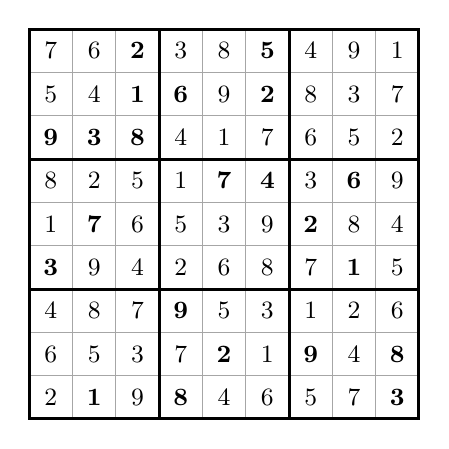
\begin{tikzpicture}[scale=0.55, every node/.style={font=\small}]
    \draw[step=1, black!35, thin] (0,0) grid (9,9);
    \draw[line width=1.1pt] (0,0) rectangle (9,9);
    \draw[line width=1.1pt] (3,0)--(3,9);  \draw[line width=1.1pt] (6,0)--(6,9);
    \draw[line width=1.1pt] (0,3)--(9,3);  \draw[line width=1.1pt] (0,6)--(9,6);
    \node at (0.5,8.5) {7};
    \node at (1.5,8.5) {6};
    \node at (2.5,8.5) {\textbf{2}};
    \node at (3.5,8.5) {3};
    \node at (4.5,8.5) {8};
    \node at (5.5,8.5) {\textbf{5}};
    \node at (6.5,8.5) {4};
    \node at (7.5,8.5) {9};
    \node at (8.5,8.5) {1};
    \node at (0.5,7.5) {5};
    \node at (1.5,7.5) {4};
    \node at (2.5,7.5) {\textbf{1}};
    \node at (3.5,7.5) {\textbf{6}};
    \node at (4.5,7.5) {9};
    \node at (5.5,7.5) {\textbf{2}};
    \node at (6.5,7.5) {8};
    \node at (7.5,7.5) {3};
    \node at (8.5,7.5) {7};
    \node at (0.5,6.5) {\textbf{9}};
    \node at (1.5,6.5) {\textbf{3}};
    \node at (2.5,6.5) {\textbf{8}};
    \node at (3.5,6.5) {4};
    \node at (4.5,6.5) {1};
    \node at (5.5,6.5) {7};
    \node at (6.5,6.5) {6};
    \node at (7.5,6.5) {5};
    \node at (8.5,6.5) {2};
    \node at (0.5,5.5) {8};
    \node at (1.5,5.5) {2};
    \node at (2.5,5.5) {5};
    \node at (3.5,5.5) {1};
    \node at (4.5,5.5) {\textbf{7}};
    \node at (5.5,5.5) {\textbf{4}};
    \node at (6.5,5.5) {3};
    \node at (7.5,5.5) {\textbf{6}};
    \node at (8.5,5.5) {9};
    \node at (0.5,4.5) {1};
    \node at (1.5,4.5) {\textbf{7}};
    \node at (2.5,4.5) {6};
    \node at (3.5,4.5) {5};
    \node at (4.5,4.5) {3};
    \node at (5.5,4.5) {9};
    \node at (6.5,4.5) {\textbf{2}};
    \node at (7.5,4.5) {8};
    \node at (8.5,4.5) {4};
    \node at (0.5,3.5) {\textbf{3}};
    \node at (1.5,3.5) {9};
    \node at (2.5,3.5) {4};
    \node at (3.5,3.5) {2};
    \node at (4.5,3.5) {6};
    \node at (5.5,3.5) {8};
    \node at (6.5,3.5) {7};
    \node at (7.5,3.5) {\textbf{1}};
    \node at (8.5,3.5) {5};
    \node at (0.5,2.5) {4};
    \node at (1.5,2.5) {8};
    \node at (2.5,2.5) {7};
    \node at (3.5,2.5) {\textbf{9}};
    \node at (4.5,2.5) {5};
    \node at (5.5,2.5) {3};
    \node at (6.5,2.5) {1};
    \node at (7.5,2.5) {2};
    \node at (8.5,2.5) {6};
    \node at (0.5,1.5) {6};
    \node at (1.5,1.5) {5};
    \node at (2.5,1.5) {3};
    \node at (3.5,1.5) {7};
    \node at (4.5,1.5) {\textbf{2}};
    \node at (5.5,1.5) {1};
    \node at (6.5,1.5) {\textbf{9}};
    \node at (7.5,1.5) {4};
    \node at (8.5,1.5) {\textbf{8}};
    \node at (0.5,0.5) {2};
    \node at (1.5,0.5) {\textbf{1}};
    \node at (2.5,0.5) {9};
    \node at (3.5,0.5) {\textbf{8}};
    \node at (4.5,0.5) {4};
    \node at (5.5,0.5) {6};
    \node at (6.5,0.5) {5};
    \node at (7.5,0.5) {7};
    \node at (8.5,0.5) {\textbf{3}};
  \end{tikzpicture}

\vspace{2mm}
{\small solution; given clues in bold}
\end{minipage}
\caption{The instance and its unique completion.}
\end{figure}

\textbf{Uniqueness.}\quad
Solving once produces \emph{a} completion. Showing it is \emph{the}
completion takes one more solve. Add the no-good cut
\[
  \sum_{(r,c)} x_{r,c,\,v^{*}(r,c)} \;\le\; 80
\]
where $v^{*}(r,c)$ is the digit found above. The left side counts how
many cells agree with that particular assignment, so the cut forbids all
81 agreeing at once while leaving every other completion available.
Re-solving with the cut returns infeasible, which proves no second
solution exists. The technique is general: it converts ``I found a
solution'' into ``I found the only solution'' for the price of one extra
solve, and the same cut repeated $k$ times enumerates the first $k$
distinct solutions of any binary program.

\newpage
%=======================================================================
\section*{EP1.\quad Total Unimodularity and the Shortest-Path Relaxation}
%=======================================================================

A matrix is totally unimodular (TU) when every square submatrix has
determinant $0$, $+1$ or $-1$. The condition applies at every order, not
only to the full matrix, and a submatrix means any selection of rows and
columns. Since each single entry is itself a submatrix of order one, all
entries of a TU matrix lie in $\{0, +1, -1\}$.

The link to integrality runs through Cramer's rule. A vertex of a
polyhedron is determined by a square nonsingular subsystem $Bx = d$, so
its coordinates are ratios of determinants with $\det(B)$ in every
denominator. When $\det(B)$ is $\pm 1$ and $d$ is integral, the vertex
has integer coordinates. Hoffman and Kruskal (1956) proved the sharp
version: for an integral matrix $A$, the polyhedron
$\{x : Ax \le b,\ x \ge 0\}$ has only integral vertices for EVERY
integral $b$ if and only if $A$ is totally unimodular. The condition is
necessary as well as sufficient.

\begin{figure}[htbp]
\centering
\begin{minipage}{0.34\textwidth}
\centering
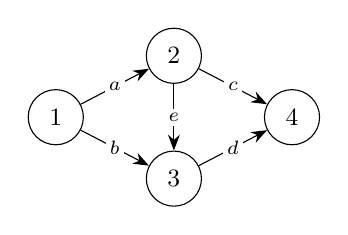
\begin{tikzpicture}[x=1.5cm, y=1.3cm]
  \node[vtx] (n1) at (0,1)   {1};
  \node[vtx] (n2) at (1,1.6) {2};
  \node[vtx] (n3) at (1,0.4) {3};
  \node[vtx] (n4) at (2,1)   {4};
  \draw[ar] (n1) -- node[lbl] {$a$} (n2);
  \draw[ar] (n1) -- node[lbl] {$b$} (n3);
  \draw[ar] (n2) -- node[lbl] {$c$} (n4);
  \draw[ar] (n3) -- node[lbl] {$d$} (n4);
  \draw[ar] (n2) -- node[lbl] {$e$} (n3);
\end{tikzpicture}
\end{minipage}
\hfill
\begin{minipage}{0.60\textwidth}
\centering
\[
  M \;=\;
  \begin{array}{c@{\;}c}
    & \begin{array}{ccccc} a & b & c & d & e \end{array} \\[2pt]
    \begin{array}{c} 1 \\ 2 \\ 3 \\ 4 \end{array} &
    \left[\begin{array}{rrrrr}
       +1 & +1 &  0 &  0 &  0 \\
       -1 &  0 & +1 &  0 & +1 \\
        0 & -1 &  0 & +1 & -1 \\
        0 &  0 & -1 & -1 &  0
    \end{array}\right]
  \end{array}
\]
\end{minipage}
\caption{A directed graph and its node-arc incidence matrix. Every
column holds exactly one $+1$ (at the tail) and one $-1$ (at the head).
That single structural fact drives the whole proof below.}
\end{figure}

\textbf{The incidence matrix is TU.}\quad
The shortest-path constraint matrix is the node-arc incidence matrix:
rows indexed by nodes, columns by arcs, $+1$ in the tail row, $-1$ in
the head row, 0 elsewhere. Each column holds exactly one $+1$ and one
$-1$. Induction on the order $k$ of a square submatrix $B$. For $k = 1$
the single entry is $0, \pm 1$ by construction. For $k > 1$, three cases
exhaust the possibilities. If some column of $B$ is all zero,
$\det(B) = 0$. If some column has exactly one nonzero entry, expanding
along it gives $\pm 1$ times a determinant of order $k - 1$, which lies
in $\{0, \pm 1\}$ by hypothesis. Otherwise every column of $B$ holds
both a $+1$ and a $-1$, so every column sums to zero, the rows of $B$
sum to the zero vector, $B$ is singular, and $\det(B) = 0$. Every case
lands in $\{0, +1, -1\}$.

\textbf{Why the relaxation is exact.}\quad
The shortest-path constraints are flow conservation, whose matrix is
exactly this incidence matrix, together with bounds $0 \le x \le 1$.
Appending an identity block for the bounds preserves total
unimodularity. The right-hand side is integral: $+1$ at $s$, $-1$ at
$t$, 0 elsewhere, with bounds 0 and 1. Hoffman and Kruskal therefore
apply, every vertex of the relaxed polytope is integral, and since a
bounded linear program attains its optimum at a vertex, the simplex
method returns a binary solution without being asked. The integer
program and its relaxation share an optimal value. This is what
Problem 2 measured: zero gap on all ten instances, no fractional arc
value anywhere, and at most one branch-and-bound node.

\textbf{Where it fails.}\quad
The property is fragile. The vertex-edge incidence matrix of an
undirected odd cycle is the standard counterexample: for a triangle it
has determinant 2, outside $\{0, \pm 1\}$. The longest-path model of
Problem 2 inherits failures of this kind, which is why its relaxation is
not exact and why branch and bound with generated constraints is
required there. Checking every square submatrix is exponential, so
usable criteria matter; Ghouila-Houri (1962) gives a characterization by
row partition, and interval matrices, network matrices and bipartite
incidence matrices are the standard TU families worth recognizing on
sight.

\newpage
%=======================================================================
\section*{EP2.\quad The Vitali Set and the Need for $\sigma$-Algebras}
%=======================================================================

Lebesgue measure on the real line is asked to satisfy four properties at
once: it assigns $\lambda([a,b]) = b - a$, it is translation invariant,
it is countably additive on disjoint sets, and it is defined for every
subset of $\mathbb{R}$. The Vitali set shows these four are jointly
inconsistent.

\textbf{Construction.}\quad
On $[0,1)$ define $x \sim y$ when $x - y$ is rational. This is an
equivalence relation, and each class is countable and dense in $[0,1)$,
so there are uncountably many classes. Using the Axiom of Choice, select
exactly one representative from each class and call the resulting set
$\nu$.

\textbf{Why $\nu$ cannot have a measure.}\quad
Enumerate the rationals in $[-1,1]$ as $q_1, q_2, \dots$ and let
$\nu_n = \nu + q_n$ be the translates. These are pairwise disjoint: if
$v + q_i = w + q_j$ then $v - w$ is rational, so $v$ and $w$ lie in the
same class, so $v = w$ by construction, so $q_i = q_j$. They also
sandwich the unit interval: every $x \in [0,1)$ differs from its class
representative by a rational in $[-1,1]$, so
\[
  [0,1) \;\subseteq\; \bigcup_{n} \nu_n \;\subseteq\; [-1,2).
\]

Suppose $\nu$ were measurable, with $\lambda(\nu) = m$. Translation
invariance gives $\lambda(\nu_n) = m$ for every $n$, and countable
additivity gives $\lambda(\bigcup_n \nu_n) = \sum_n m$. Two cases, both
impossible. If $m = 0$ the union has measure 0, yet it contains $[0,1)$
of measure 1. If $m > 0$ the union has measure $\infty$, yet it sits
inside $[-1,2)$ of measure 3. No value of $m$ works, so $\nu$ is not
Lebesgue measurable.

\textbf{What has to be given up.}\quad
The contradiction used all four properties, so at least one must go.
Normalization is what measure means and cannot go. Translation
invariance is the defining symmetry of length. Countable additivity is
what separates measure theory from finitely additive content and is what
makes limit theorems work. The remaining property is the one abandoned:
a measure need not be defined on every subset. Note that the
construction requires the Axiom of Choice, and this is not incidental.
Solovay (1970) showed that ZF with dependent choice is consistent with
the statement that every set of reals is Lebesgue measurable, so no
explicit non-measurable set can be exhibited without some form of
choice.

\textbf{Why this forces $\sigma$-algebras.}\quad
Restricting the domain is only coherent if the restricted collection is
closed under the operations measure theory actually performs. Those
operations are complementation and countable union, and closure under
exactly those is the definition of a $\sigma$-algebra $\mathcal{F}$.
This is why a probability space is the triple
$(\Omega, \mathcal{F}, \mathbb{P})$ rather than just a sample space and a
number-valued function: $\mathcal{F}$ names which events are permitted
to have probabilities. Countable rather than finite closure is
essential, because limits, tail events and the convergence theorems all
require countably many operations.

\textbf{Consequence for this course.}\quad
Expectation is a pairing between a random variable and a measure, and
the pairing is only defined when both live on the same
$\sigma$-algebra: the variable must be $\mathcal{F}$-measurable and the
measure defined on $\mathcal{F}$. Every construction that follows
depends on this. Value-at-Risk needs the distribution function to be
well defined; Conditional Value-at-Risk needs conditional expectation,
which is defined as a Radon--Nikodym derivative with respect to a
sub-$\sigma$-algebra and has no meaning without one; distributionally
robust optimization ranges over a set of probability measures, which
presupposes a fixed $\mathcal{F}$ on which they are all defined. The
Vitali set is the reason that bookkeeping is mandatory rather than
pedantic.

\end{document}
